\documentclass{article}
\usepackage{graphicx} % Required for inserting images

\usepackage{amsmath}
\usepackage{hyperref}
\usepackage{amsfonts}
\usepackage{soul}
\usepackage{xcolor}
\usepackage{moresize}

%\title{SGCD: Q1 was never solvable (unfinished draft)}

\title{\st{SGCD: Q1 Investigation Results}\\The SiIvaGunner Calculation Convention Crisis: a Q1 Postmortem}
\author{guineawheek, 4mbr0s3 2, 91124V}
\date{January 2025}

\begin{document}

\maketitle

Note: This has not been peer reviewed yet.
Please don't share this yet until this has been formally addressed with the author (who will not be named on this document, though it's very easy to look up on the Discord server) of the original problem.

\begin{abstract}
In this paper, we present a postmortem of Question 1 of one of the final steps in the SiIvaGunner RES:PH ARG! which involved \textbf{math} (more specifically, the \textbf{attention} mechanism in machine learning).
\\\\
\noindent We discuss the background of the problem, mistakes in the problem formulation and solution (from both the solvers and, potentially, the problem author), and why ARG solvers ultimately could not get the numbers to line up trying to solve this problem in the ARG. 
\\\\
We conclude that the ultimate root cause stem from pedagogical decisions that the YouTube channel 3Blue1Brown (hereafter "3b1b") run by Grant Sanderson made to explain the attention mechanism which contrast with the mathematical conventions used by the original authors of the "Attention is All You Need" paper \cite{aiayn} and that the solution assumed usage of Sanderson's formulation.
\\\\
Hence, the question has not, in fact, given solvers all that they needed.
\end{abstract}

\section{Context}
\textbf{If you're already very familiar with the RE:SPH ARG! and SiIvaGunner Classified Documents (SGCD), please skip this section.}

\vspace{1cm}

As part of the recent SiIvaGunner ARG (later revealed to be named RE:SPH ARG!), 10 puzzles in a \href{https://drive.google.com/drive/folders/1oihJsu_rC_jLYnrxSGKl3X3br3DS8OS1}{Google Drive folder}, inspired by Harvard University's CS50x Puzzle Day (the "x" means online), were presented to ARG solvers.

Only 8 of the 10 problems needed to be solved in order to progress.

After 3 days, all other problems have been solved with concrete explanations except for Question 1. Other solvers had brute-forced the answer to be "mat", but Q1-dedicated solvers still continued to attempt to derive an explanation.

As the other questions in this step of the ARG all had text answers that related with their problem (e.g. "chess" for a rather complicated chess puzzle, much to the chagrin of its solver), some  have speculated "\text{mat}" to mean "\textbf{mat}h", or "\textbf{mat}rix", or "\textbf{Mat}t Parker", etc.
\\\\
Here's Question 1, which is the question (in question) that made us question our sanity:

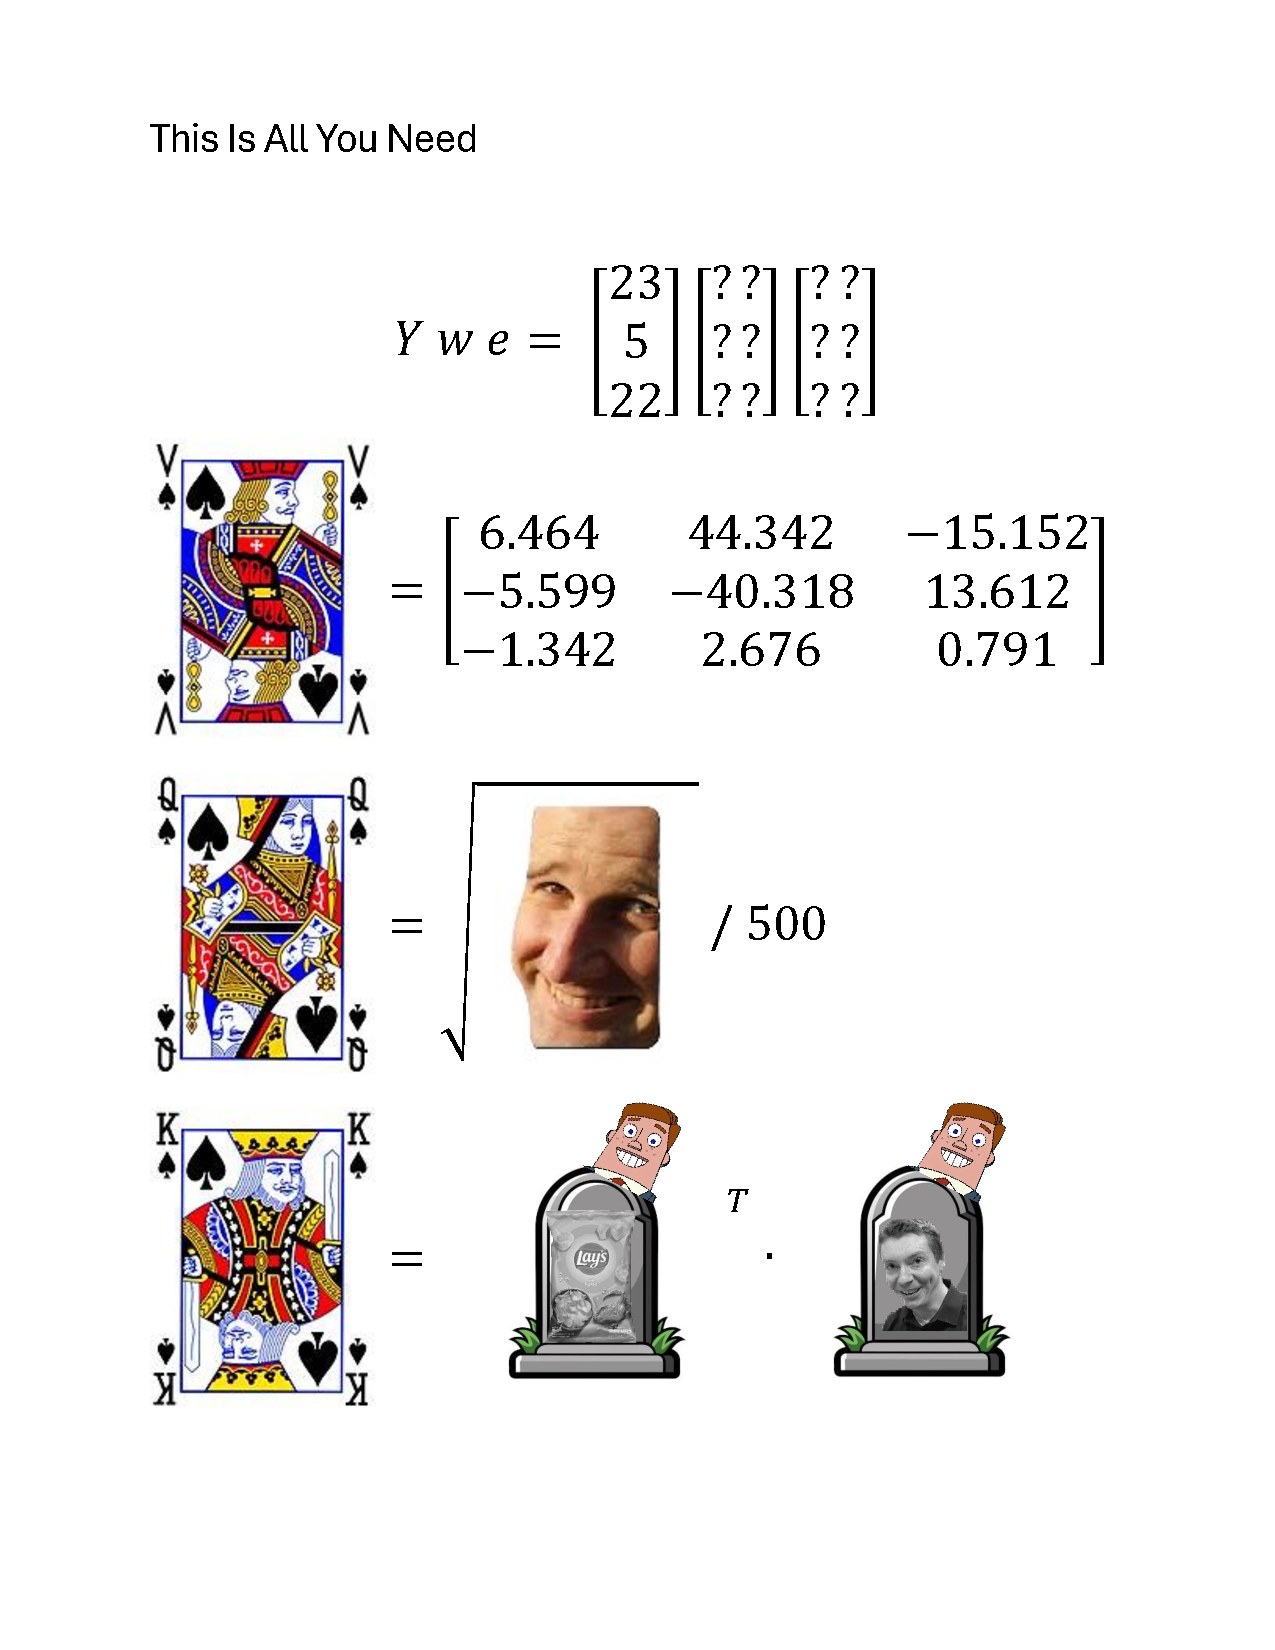
\includegraphics[width=11cm]{1.pdf}

Solvers were quick to solve matrices $Q$ and $K$. 

Matrix $Q$ was derived by taking the \href{https://en.wikipedia.org/wiki/Magic_square#Parker_square}{Parker square}, doing an element-wise square root followed by an element-wise division by 500.

Matrix $K$ involves matrix arithmetic derived from vectors that are references to a recent SiIvaGunner lore event, although the problem's formulation contains an error elaborated on later.

Solvers, stuck on what to do with $Q$, $K$, and $V$, eventually figured out that the problem's title is a hint to the "Attention Is All You Need" paper and the Attention mechanism.

However, it took some time before people figured out $Ywe$, the 3 × 3 matrix at the top consisting of column vectors \href{https://siivagunner.fandom.com/wiki/Y_-_Kero_Blaster}{$Y$}, \href{https://siivagunner.fandom.com/wiki/W_-_Deltarune}{$w$}, and \href{https://siivagunner.fandom.com/wiki/Main_Theme_-_e}{$e$}, which corresponded to the upload dates of specific SiIva rips with single-letter track names.

When they did, it seemed like solving the puzzle was easy: use $Ywe$ as an input matrix and use $Q$, $K$, and $V$ as weights to calculate the $Q$, $K$, and $V$ needed for the Attention function.

Despite having \textit{all} that they need... People still didn't figure it out.

When the problem author released a solution\footnote{The solution was first discovered in a \href{https://docs.google.com/document/d/1GnD42mGr2TM23O65WiNPZae3WjgZuFj-4iYNhHk_TVg}{Google Doc link} hidden in the unobfuscated source code of a Balatro mod that immediately followed these puzzles. Later, a more thorough solution that included calculations was posted as a \href{https://discord.com/channels/220275955329925120/1319443290428280855/1331873078321610825}{.txt} on the Official SiIvaGunner Fan Server.} after the ARG ended, we took the liberty to verify how it was done.

As it turns out, it seems that the way the solution calculated the attention is... well, it's not \textit{wrong} per se, but it assumes one uses Grant Sanderson's column-vector-focused formulation of attention, and \emph{not} the row-vector-focused formulation from the original paper.

\section{The intended solution}

The following steps directly follow the \verb|.txt| file posted on the SiIvaGunner Discord.\\\\

Once $V$, $Q$, and $K$ are calculated, we first collate our $Y$, $w$, and $e$ matrices into a data matrix $X$ as such:
\begin{align*}
    X = \begin{bmatrix} | & | & |\\Y & w & e\\| & | & |\\\end{bmatrix}
    = \begin{bmatrix}23 & 9 & 15\\5 & 8 & 1\\22 & 22 & 17\end{bmatrix}
\end{align*}
From this, we calculate our attention matrix $A$ and goal matrix $G$ as such:
\begin{align*}
    Q &= W_QX\\
    K &= W_KX\\
    V &= W_VX\\
    d_k &= 3\\
    A &= V \cdot \mathbf{softmax}_\text{col}\left(\frac{K^TQ}{\sqrt{d_k}}\right)\\
    G &= X + A\\
    &= \begin{bmatrix}
    21.98558375 & 15.98495201 & 13.98759627 \\ 
     8.00513334 &  4.00556591 &  3.00371168 \\ 
    23.00109975 & 22.00119296 & 24.00077455 \\ 
    \end{bmatrix}\\
    &\approx \begin{bmatrix}
    22 & 16 & 14 \\
     8 &  4 &  3 \\
    23 & 22 & 24 \\
    \end{bmatrix}
 \end{align*}
where $\mathbf{softmax}_\text{col}$ performs the softmax operation over only the columns.

The columns of the integer-rounded value of $G$ correspond to upload dates of three other single-character-associated rips, which spell out "mat".

You can find the computation for this solution in this Google Colab.

\vspace{1cm}
Did you see it?\footnote{4k6VFcaFeC0}
\vspace{1cm}

That Attention function is (on the surface) \emph{very} different from the original paper! Not only that, but we apparently have to left-multiply by the weights $Q$, $K$, and $V$ instead of right-multiply (like most implementations do!)

Does this mean that the official solution is wrong? This was our initial guess, but, as it turns out, the paper did \emph{not} give us all we needed...

\section{The Calculation Convention Crisis}
The original Scaled Dot-Product Attention function in the research paper "Attention Is All You Need" by Vaswani et al. \cite{aiayn}, as do pretty much all other online examples, code or otherwise essentially formulate the equation like \textit{this:}
\[\text{Attention}(Q, K, V) = \mathbf{softmax}_{\text{row}}\left(\frac{QK^T}{\sqrt{d_k}}\right)V\]

Additionally, $Q$, $K$, and $V$ are computed as $XW_Q$, $XW_K$, and $XW_V$ respectively. 

This was the equation Q1 solvers found and attempted to use, which was \textbf{not} the formulation that the official Q1 solution used as it followed a formulation from a \href{https://www.youtube.com/watch?v=eMlx5fFNoYc}{3Blue1Brown video on the subject}\footnote{The exact video that the .txt cites is \emph{Attention in transformers, step-by-step | DL6} by 3Blue1Brown: \href{https://www.youtube.com/watch?v=eMlx5fFNoYc}{https://www.youtube.com/watch?v=eMlx5fFNoYc}}.


Astute observers would note that in order for the data matrix $X$ to be correct, it would need to be transposed from the intended solution as to have
\[
X^T = \begin{bmatrix}
- & Y^T & - \\
- & w^T & - \\
- & e^T & - \\
\end{bmatrix}
\]
instead as the original paper assumes that input data points are row vectors -- not something that would've been necessarily obvious to ARG solvers. 

But this alone would not have been sufficient to derive the correct solution as the Q, K, and V weights matrices derived from the problem statement would also need to be transposed for the original paper's equation to yield a correct solution.

These are all things that would not be apparent or even necessarily inferrable unless one was (a) aware of the 3b1b video and (b) aware that it was at odds at everything else and (c) knew why it would be at odds with the results, as without it one would reasonably assume that the values of Q, K, and V matrices would be correct for the original paper's formulation.


\subsection{Columns vs. rows}

The reason for this discrepancy between the 3b1b video and the original Attention is All You Need paper is due to differing conventions on how to represent the data vectors.

Grant Sanderson chose to represent data inputs and outputs as column vectors, whereas the original paper and basically everyone else in machine learning assumed they would be row vectors.

While someone \textit{did} link the 3b1b video, it was somewhat dismissed out of hand as solvers were already fixated on the original paper's contents.


\subsection{A simple algebraic proof \footnotesize{(by 4mbr0s3 2)}}
With the research paper alone, which utilized row vectors, there's \textit{no way} we could have possibly known that $W_Q$, $W_K$, and $W_V$ used column vectors and that they needed to be transposed into row vectors to work with the paper's attention function.

The only "hint" that could've told solvers that all of these were column vectors was with the top matrix $X = Ywe$, which had $Y$, $w$, and $e$ in columns. The problem with this is that $W_Q$, $W_K$, and $W_V$ would've also needed to be transposed into row vectors, and the problem's hint toward the paper implied that $X$
should just be right-multiplied by the weight matrices. An extra transposition step for several matrices here \emph{deviates} from the paper.

In retrospect, both weight and input matrices needed to be transposed into row vectors to work with the paper's function:

\begin{align*}
    Q_R = X^TW_Q^T = (W_QX)^T = Q_C^T\\
    K_R = X^TW_K^T = (W_KX)^T = K_C^T\\
    V_R = X^TW_V^T = (W_VX)^T = V_C^T\\
\end{align*}

The following is a simple algebraic proof that this transposition from column to row vectors would've actually yielded the same function as the paper:

\begin{align*}
    \mathbf{softmax}_\text{row}\left(\frac{Q_RK_R^T}{\sqrt{d_k}}\right) V_R + X_R &= \left(V_C \cdot \mathbf{softmax}_\text{col}\left(\frac{K_C^TQ_C}{\sqrt{d_k}}\right)\right)^T + X_C^T\\
    &= \mathbf{softmax}_\text{row}\left(\frac{(K_C^TQ_C)^T}{\sqrt{d_k}}\right)V_C^T + X_C^T\\
    &= \mathbf{softmax}_\text{row}\left(\frac{Q_C^TK_C}{\sqrt{d_k}}\right)V_C^T + X_C^T\\
    &= \mathbf{softmax}_\text{row}\left(\frac{Q_RK_R^T}{\sqrt{d_k}}\right)V_R + X_R\\
\end{align*}

This also explains our previous (incorrect) qualm about the matrix multiplication being flipped in the solution, which, as seen above, is explained by matrix transposition properties.

\subsection{Why would 3Blue1Brown do this to us? \footnotesize{(by Guinea)}}
Grant used column vectors for pedagogical reasons, and because he likes to visualize the relevant vectors as columns.
\begin{figure}[ht]
    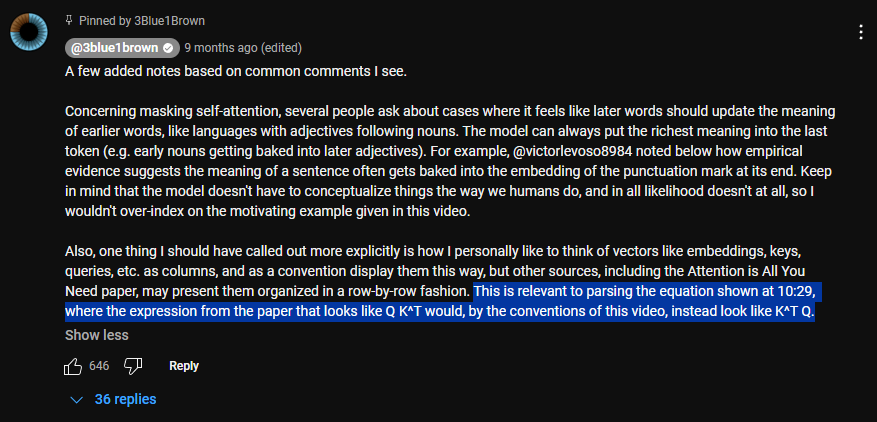
\includegraphics[width=\textwidth]{grant_comment.png}
    \caption{Grant's pinned comment in his Transformers video}
\end{figure}


As an educational mathematics YouTube channel with a particular focus on teaching linear algebra, one generally uses column vectors when teaching linalg.
It makes it a lot easier to visualize the Q, K and V weights matrices transforming input and output vectors in and out of the embeddings vector space.\footnote{It's genuinely wild that we have technology that could tell you that "midislap rip" is conceptually closer to "low quality" or "rejected submission" than to the phrase "high quality submission." We've managed to quantify human language and how concepts expressed in it all relate to each other. This is the future we live in.}
And indeed, it's reasonable to assume column vectors for most domains as it's generally easier to reason about $Ax$ versus $x^TA$.
It takes up less horizontal space to write out and is more space-efficient to notate with.

\subsection{AI ruins everything \footnotesize{(by Guinea)}}
However, the original paper authors were machine learning researchers.
In data science/statistics/ML/what have you, you generally want your input data points to be row vectors (or row "tensors", I guess).
This poses a number of advantages. When you import tables from Excel sheets, CSV files, SQL databases, or really anywhere else, your data points tend to come in rows.
When you are mucking around in Jupyter notebooks, having your data points be individual rows means that if you want to get the Nth data point, you'd likely pull it using \texttt{pt\_N = df[N]}. 

This means, however, that in practice all your code is going to assume row vectors. 
And normally, we wouldn't really care much about the actual values of the Q, K, and V weights because they would get trained on via backpropogation but in this ARG question they are hardcoded values that we solve for, so how they are transposed actually does matter.



%\subsection{Variable Solutions}
%
%As you've seen, the original problem had some... unique ways of expressing the variables needed for the Attention mechanism.
%
%The following are the correct solutions to variables and matrices for the problem:
%
%\[ Ywe = \begin{bmatrix}
%  23 & 9 & 15\\ 
%  5 & 8 & 1\\
%  22 & 22 & 17
%  \end{bmatrix}\]
%
%\[ W_V = \begin{bmatrix}
%  
%  \end{bmatrix}\]



\section{Nitpick: Outer products vs. dot products \footnotesize{\\(by Guinea)}}

That's not to say that the problem statement is fully error-free, however, as the intended calculation of the K matrix is incorrect.

The derivation of the $K$ matrix comes from the death points of Omega Lays and the Numberphile/James Grime in the Coordinate Plane during the \href{https://siivagunner.fandom.com/wiki/E%E2%88%A9%CE%A9}{$\mathbf{e} \cap \Omega$} SiIvaGunner sub-arc. These positions, $K_\text{lays}$ and $K_\text{grime}$ are at:

\[ K_\text{lays} = \begin{bmatrix} -6.9\\0\\9.8\end{bmatrix} \]
\[ K_\text{grime} = \begin{bmatrix} 3.3\\-2.2\\0.9\end{bmatrix} \]

and this column vector notation is what the question author's solution uses.\footnote{It could be debated, especially given their horizontal presentation in the $\mathbf{e} \cap \Omega$ series, that the coordinates were meant to be row vectors. I (Guinea) personally disagree given the use of column vectors everywhere else and the use of column vectors in a published solution, but we tried both during the ARG anyway.}

With Norm attached to their graves in the problem statement (implying we should normalize the lays and grime vectors), we can infer that:
\begin{align*}
    K &= \frac{1}{\|K_\text{lays}\|}K_\text{lays}^T \cdot \frac{1}{\|K_\text{grime}\|}K_\text{grime}\\
    &= \frac{1}{\|K_\text{lays}\| \cdot \|K_\text{grime}\|}K_\text{lays}^T K_\text{grime}\\
    &= \frac{1}{\|K_\text{lays}\| \cdot \|K_\text{grime}\|} 
    \begin{bmatrix} -6.9 & 0 & 9.8\end{bmatrix}
    \begin{bmatrix} 3.3\\-2.2\\0.9\end{bmatrix}\\
    &\approx -0.2862
\end{align*}
But that's not what the author got though, as they instead took the \href{https://en.wikipedia.org/wiki/Outer_product}{\textbf{outer product}} rather than the dot product, commonly notated for column vectors as $\mathbf{ab}^T$ rather than $\mathbf{a}^T\mathbf{b}$:
\begin{align*}
    K_\text{sol} &= \frac{1}{\|K_\text{lays}\| \cdot \|K_\text{grime}\|}K_\text{lays} K_\text{grime}^T\\
    &= \frac{1}{\|K_\text{lays}\| \cdot \|K_\text{grime}\|} 
    \begin{bmatrix} -6.9 \\ 0 \\ 9.8\end{bmatrix}
    \begin{bmatrix} 3.3 &-2.2&0.9\end{bmatrix}\\
    &\approx \begin{bmatrix}
    -0.46713506 &  0.31142337 & -0.12740047 \\
     0          &  0          &  0          \\
     0.66346719 & -0.44231146 &  0.1809456  \\
    \end{bmatrix}
\end{align*}
We, the ARG solvers, figured that this could've been a possibility especially since having a K matrix that was actually just a scalar would've been out of place with the Q and V matrices which were 3x3, and so attempted computation with both.

\section{Guinea's conclusions}
The original solution thus isn't really "wrong" (outer products aside), but entirely hinges on specifically doing the 3b1b method.
Grant Sanderson's quest to explain linear algebra to the masses managed to create a turbonoaka

I wonder if you could animate a boss fight with a chicken nugget in manim\footnote{also consider reading the puella magi madoka magica fanfiction "to the stars"}

\newpage
\section{4mbr0s3 2's conclusions}

\\

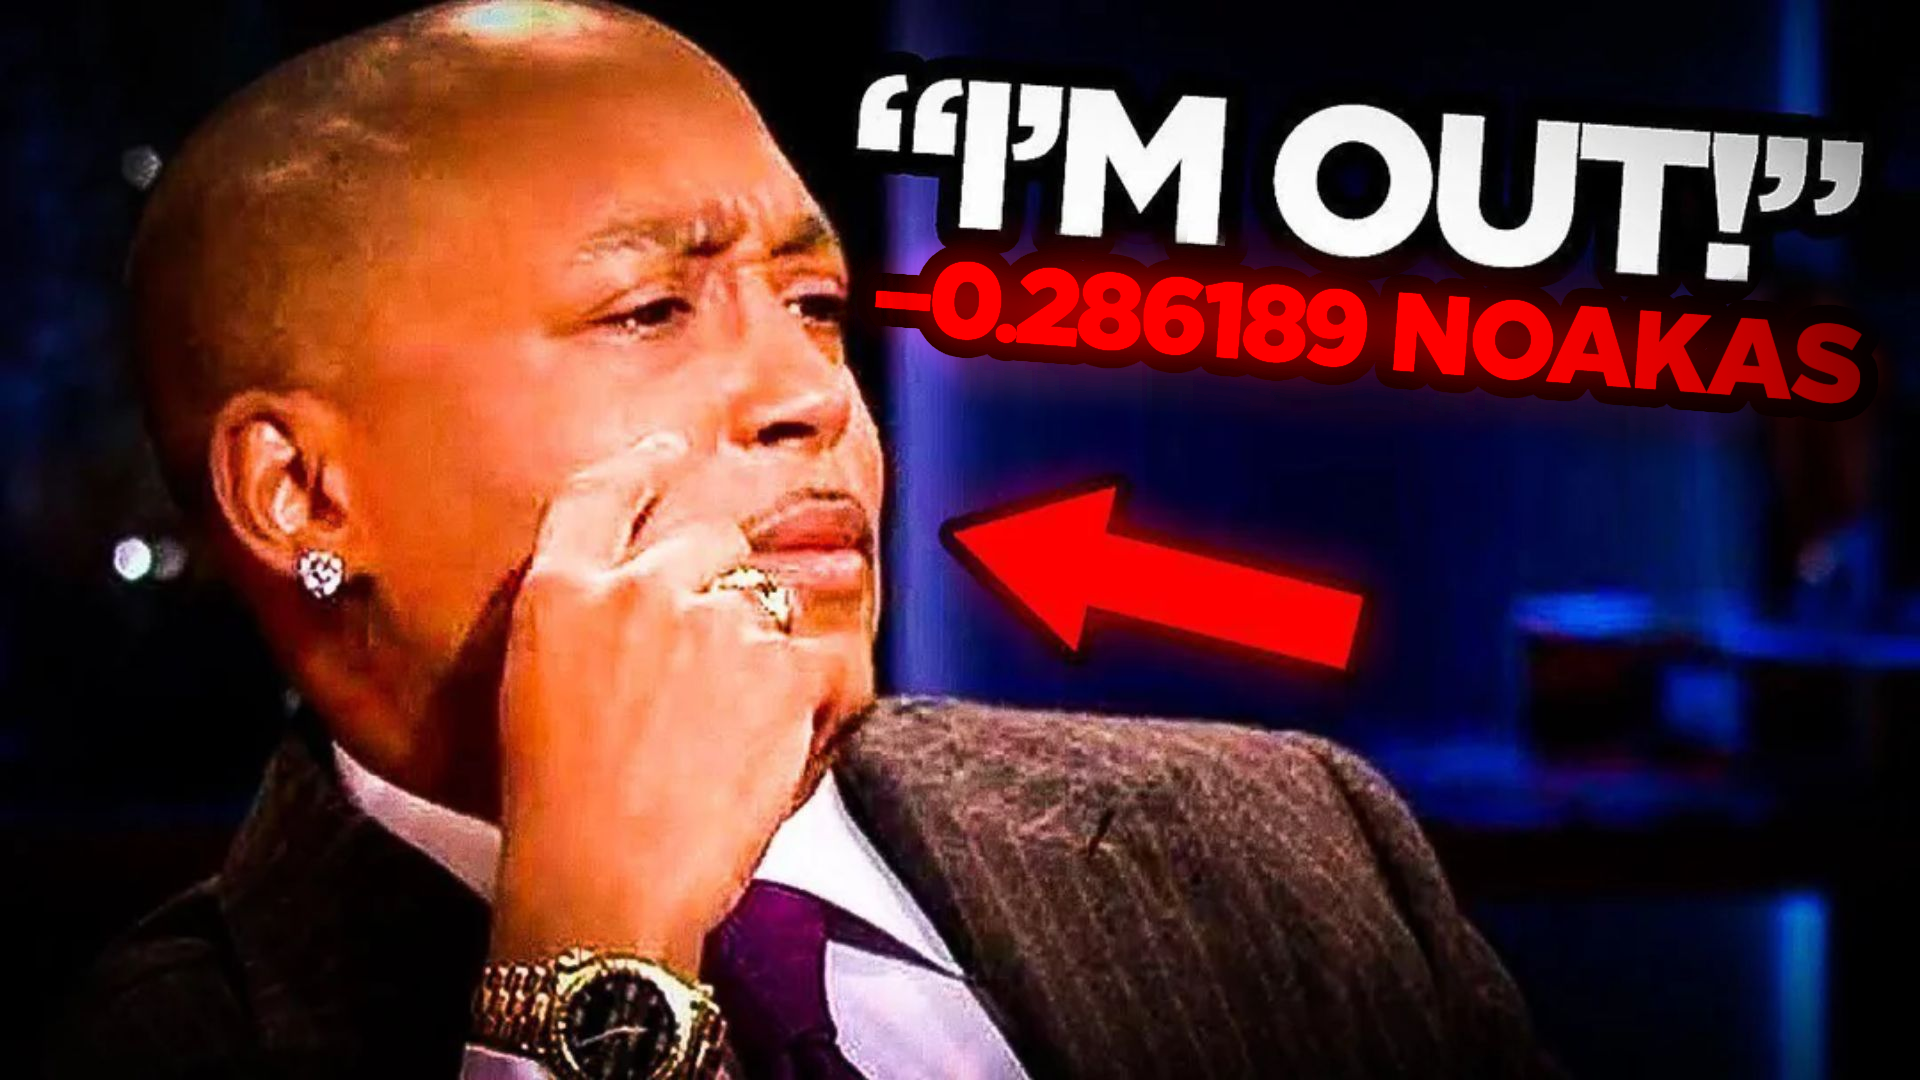
\includegraphics[width=\textwidth]{im_out_2.png}

\section{91124V's conclusions}
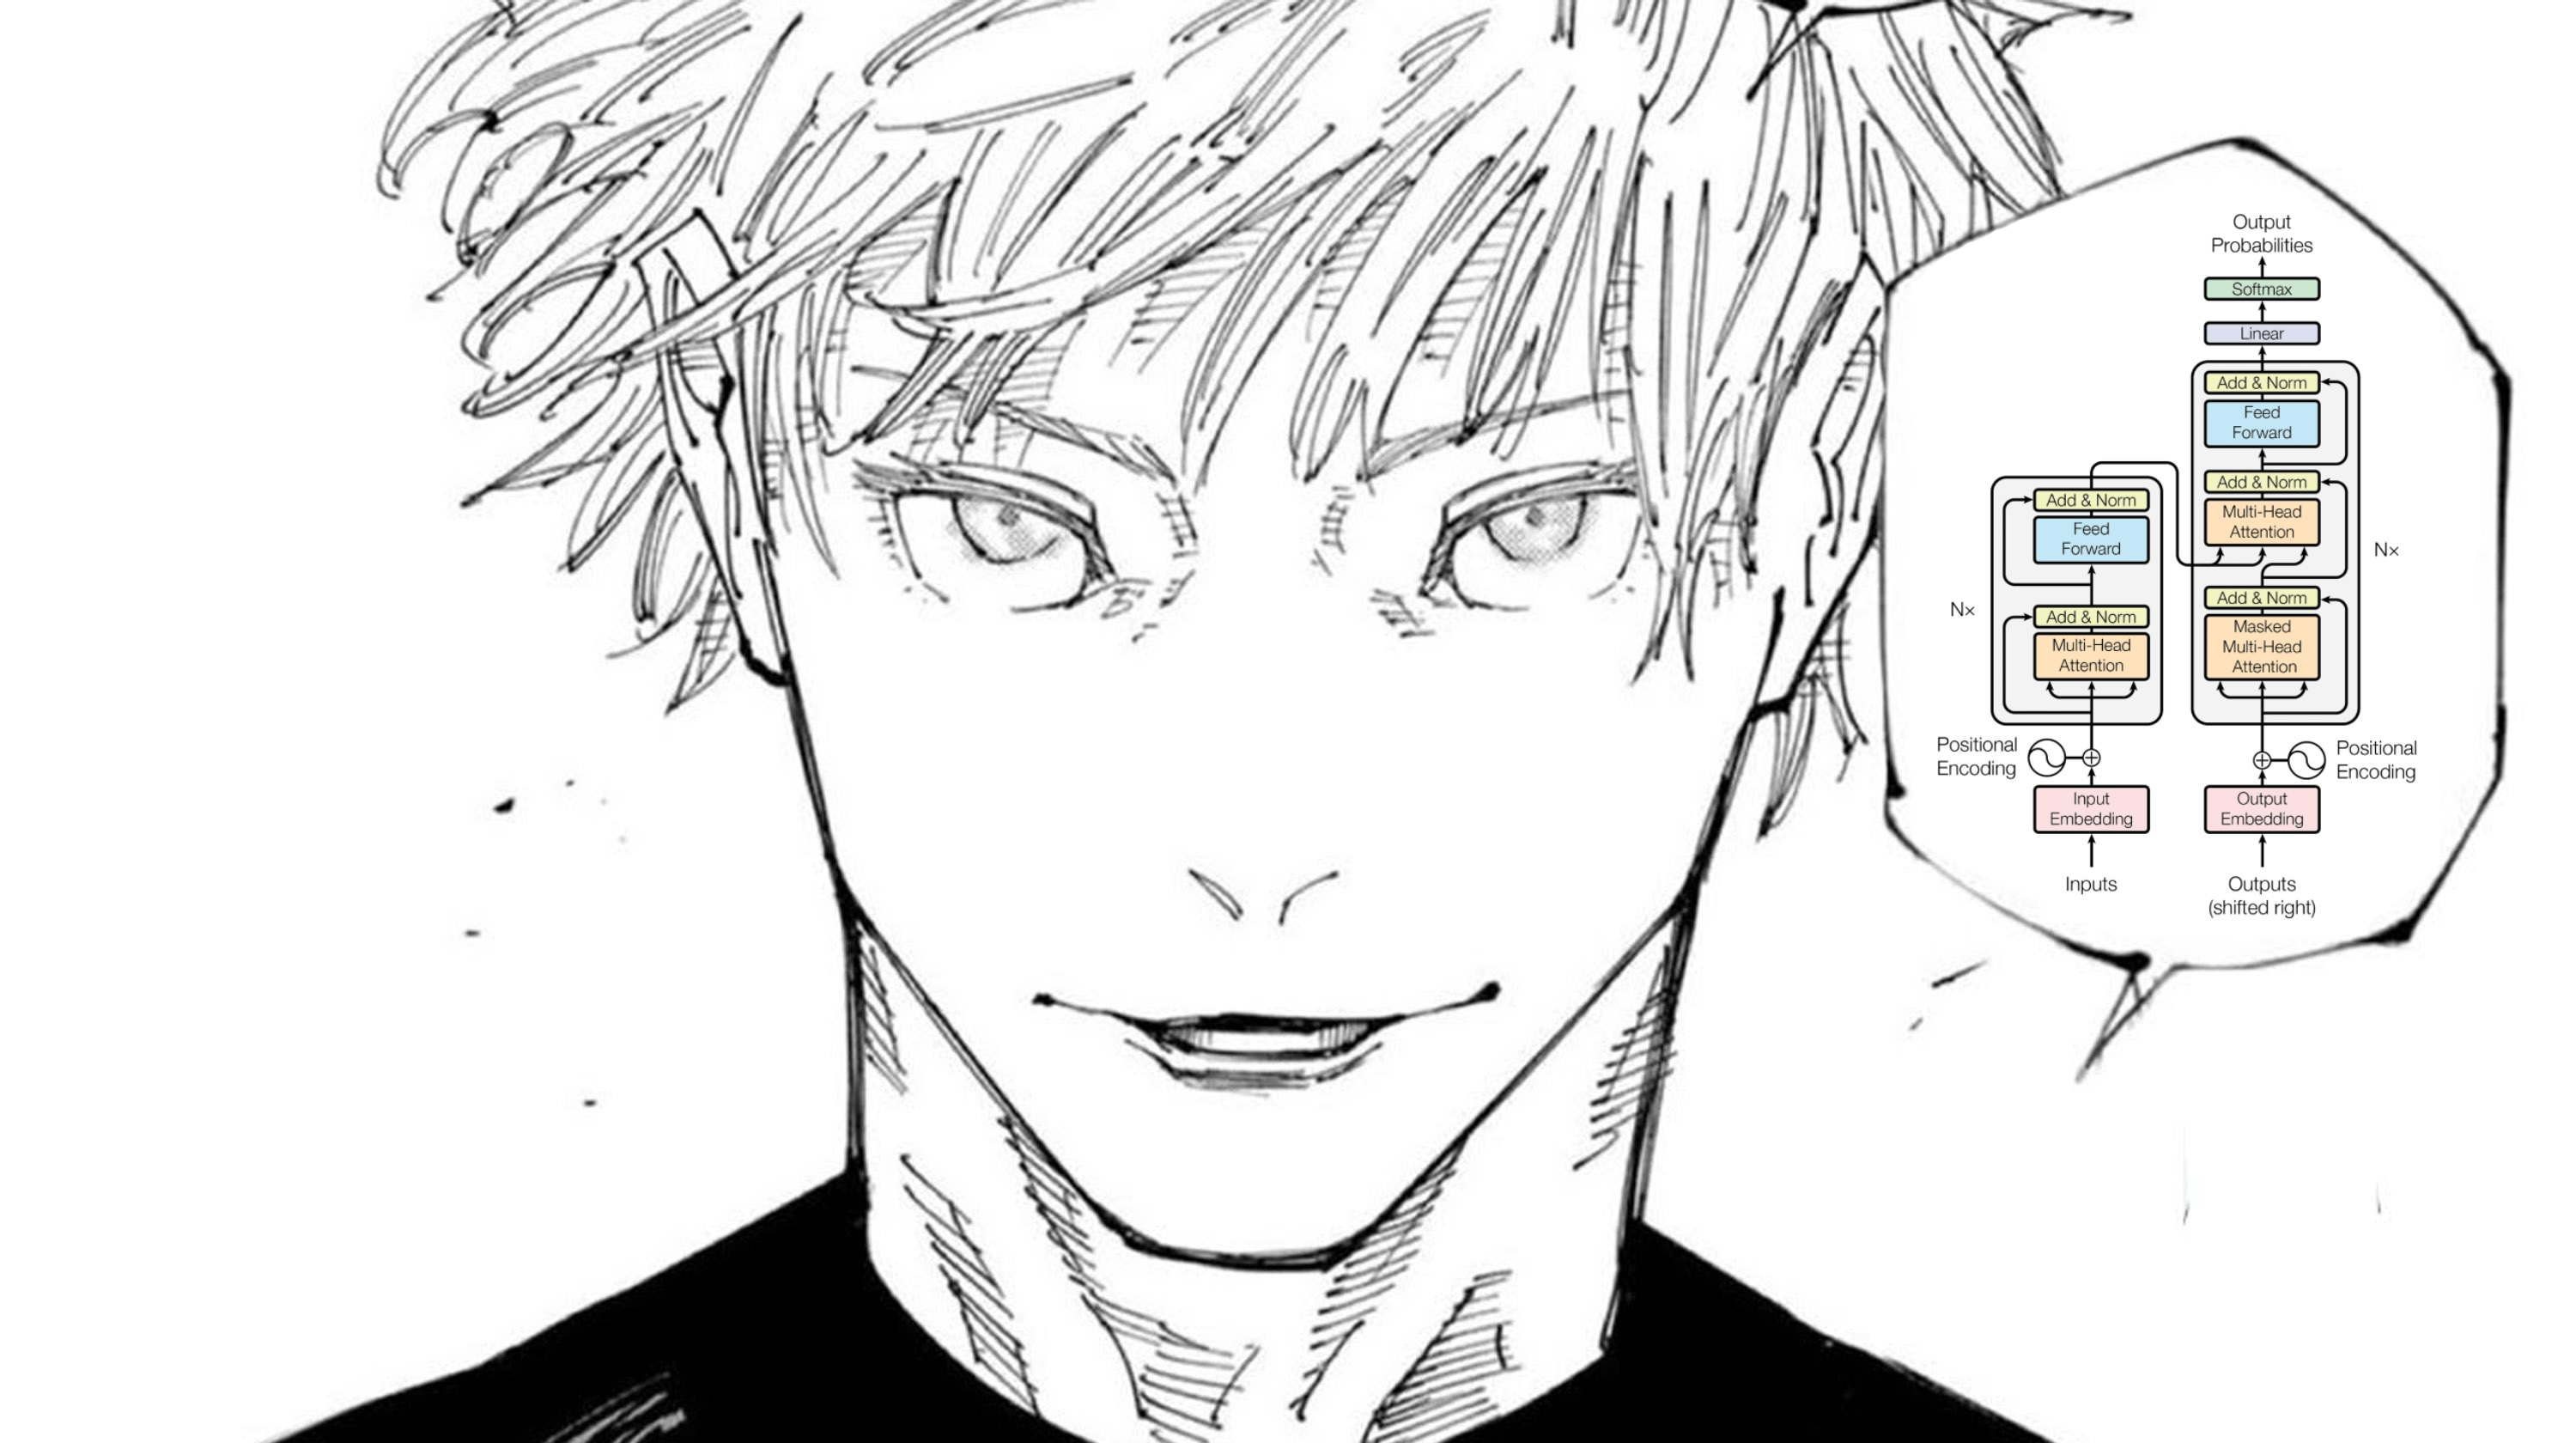
\includegraphics[width=\textwidth]{dsaf.jpg}

\newpage



\setcounter{section}{8}
\section{Conclusion}

All in all, it seems that the row-vector interpretation of the column-vector matrices and the consequent lack of coherence in any result of the row-vector calculations was ultimately the reason there wasn't enough attention paid to this problem.

\vspace{3 cm}

But we have one last question...

\vspace{3 cm}

{
\fontsize{0}{0}\selectfont
\color{white}
MiSide: Chapter "Reading Books, Destroying Glitches", Mila's first line after 3rd glitch (English localization)
}
 

\begin{thebibliography}{9}
\bibitem{aiayn}
Ashish Vaswani and Noam Shazeer and Niki Parmar and Jakob Uszkoreit and Llion Jones and Aidan N. Gomez and Lukasz Kaiser and Illia Polosukhin (2023) \emph{Attention Is All You Need}.

\end{thebibliography}

\section{Solution Code}
Our solution comparing the method used by the paper and the author's solution is documented in \href{https://colab.research.google.com/drive/1Q0nNQ7fgpgReLvLv7iyQmWx6opQ1Zw76?authuser=1}{this} Google Colab notebook. 

\section{Special Thanks}
NeoTheSomething, SmallBlue, edith (hartmann.s.youkai.girl), Pikachuness, Grant Sanderson, Daymond John, anyone else who struggled with us on this problem, and everyone else who \emph{greatly} motivated us by posting anything along the lines of "Problem 1 will never be solved."

\end{document}
